\documentclass[12pt]{article}
\usepackage{times} 			% use Times New Roman font

\usepackage[margin=1in]{geometry}   % sets 1 inch margins on all sides
\usepackage[hidelinks]{hyperref}               % for URL formatting
\usepackage[pdftex]{graphicx}       % So includegraphics will work
\setlength{\parskip}{1em}           % skip 1em between paragraphs
\usepackage{datetime}
\usepackage[small, bf]{caption}
\usepackage{listings}               % for code listings
\usepackage{xcolor}                 % for styling code
\usepackage{multirow}
\usepackage{subcaption}     % for subfigures

%\setlength\intextsep{1.69cm} 

%New colors defined below
\definecolor{backcolour}{RGB}{246, 246, 246}   % 0xF6, 0xF6, 0xF6
\definecolor{codegreen}{RGB}{16, 124, 2}       % 0x10, 0x7C, 0x02
\definecolor{codepurple}{RGB}{170, 0, 217}     % 0xAA, 0x00, 0xD9
\definecolor{codered}{RGB}{154, 0, 18}         % 0x9A, 0x00, 0x12

%Code listing style named "gcolabstyle" - matches Google Colab
\lstdefinestyle{gcolabstyle}{
  basicstyle=\ttfamily\small,
  backgroundcolor=\color{backcolour},   
  commentstyle=\itshape\color{codegreen},
  keywordstyle=\color{codepurple},
  stringstyle=\color{codered},
  numberstyle=\ttfamily\footnotesize\color{darkgray}, 
  breakatwhitespace=false,         
  breaklines=true,                 
  captionpos=b,                    
  keepspaces=true,                 
  numbers=left,                    
  numbersep=5pt,                  
  showspaces=false,                
  showstringspaces=false,
  showtabs=false,                  
  tabsize=2
}

\lstset{style=gcolabstyle}      %set gcolabstyle code listing

% to make long URIs break nicely
\makeatletter
\g@addto@macro{\UrlBreaks}{\UrlOrds}
\makeatother

% for fancy page headings
\usepackage{fancyhdr}
\setlength{\headheight}{13.6pt} % to remove fancyhdr warning
\pagestyle{fancy}
\fancyhf{}
\rhead{\small \thepage}
\chead{\small CS 532, Fall 2024} 
\lhead{\small HW 1, Parman}  % EDIT THIS, REPLACE # with HW number

%-------------------------------------------------------------------------
\begin{document}

% EDIT THE ITEMS HERE
\begin{centering}
{\large\textbf{HW 1 - Web Science Intro}}\\ 
Jenah Parman\\
September 15, 2024\\
\end{centering}

%-------------------------------------------------------------------------

% The * after \section just says to not number the sections
\section*{Q1}

\begin{figure}[!ht]
    \centering
    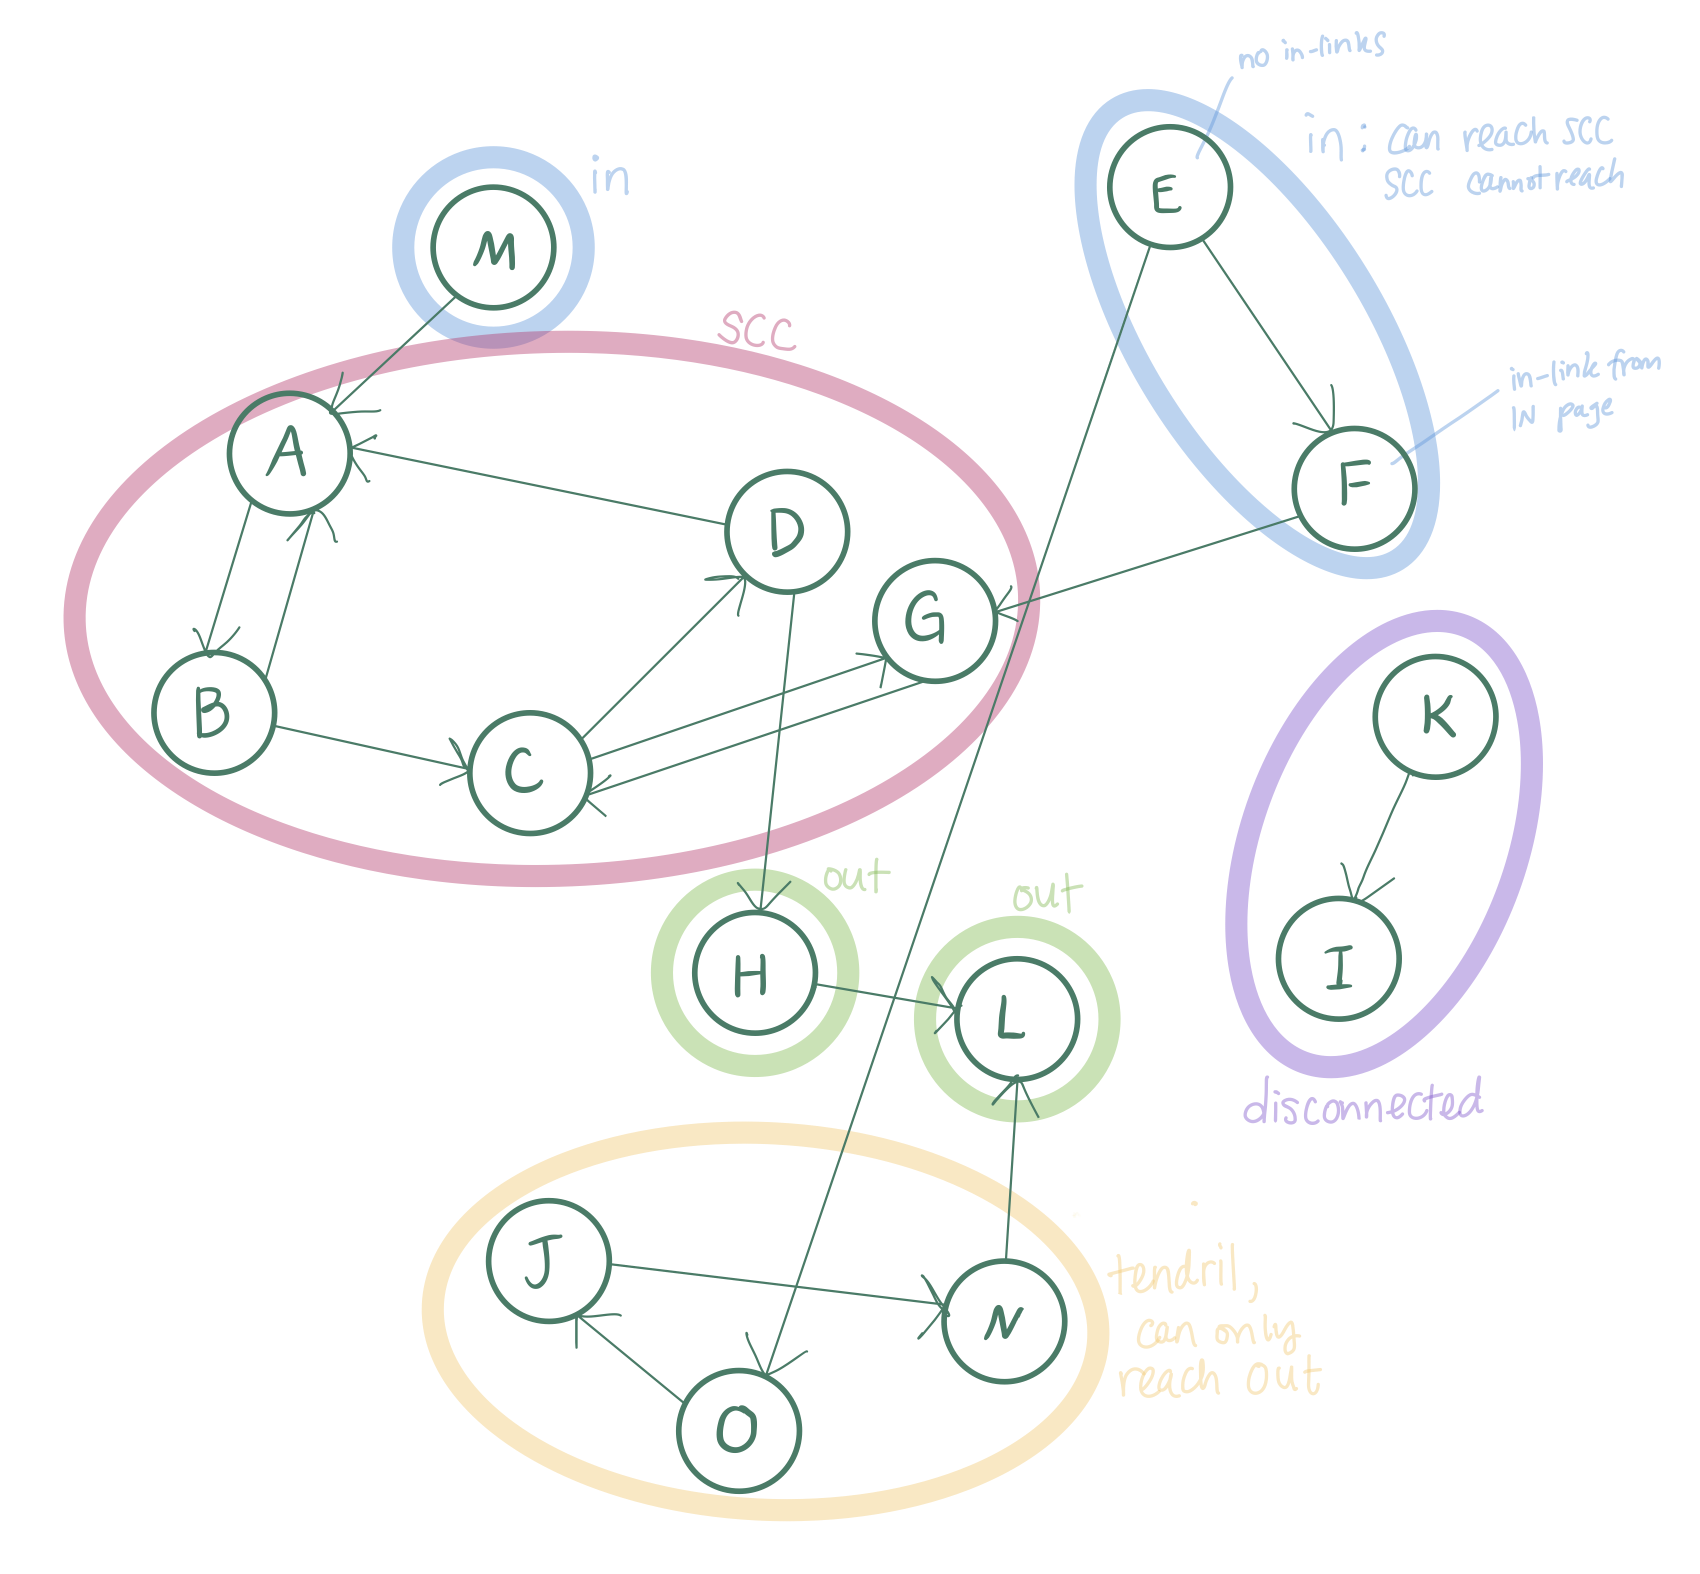
\includegraphics[height=0.5\linewidth]{directedgraph.png}
    \caption{Directed Graph of Node Relations}
    \label{fig:directedgraph}
\end{figure}

In this directed graph, the nodes are categorized based on their connectivity:

\begin{itemize}
    \item Strongly Connected Component (SCC): Nodes A, B, C, D, and G form the SCC. This component is characterized by the fact that every node is reachable from every other node in the group, creating a cycle.
    \item IN Component: Nodes M, E, and F belong to the IN component. These nodes can reach the SCC but are not reachable from it, indicating they only have outgoing paths to the SCC.
    \item OUT Component: Nodes H and L are in the OUT component. They can be reached from the SCC but cannot return to it, indicating they are endpoints of paths originating from the SCC.
    \item Tendrils: Nodes J, N, and O are classified as tendrils. Tendrils are connected to nodes in the OUT component but do not directly connect to the SCC.
    \item Disconnected Component: Nodes K and I are completely disconnected from the rest of the graph, meaning they have no direct or indirect path to or from the SCC or other components.
\end{itemize}


\section*{Q2}

a) First, load the webpage at the URI in your web browser. The result should show the "User-Agent" HTTP request header that your web browser sends to the web server. Take a screenshot to include in your report.

\begin{figure}[!ht]
    \centering
    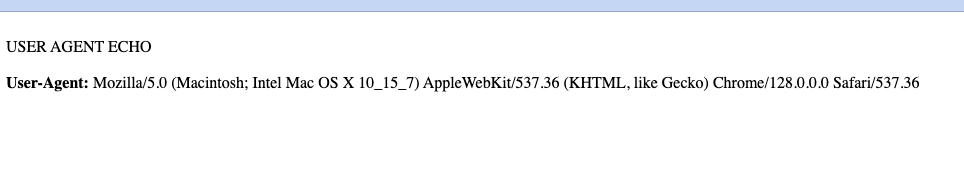
\includegraphics[width=0.5\linewidth]{q2_1.png}
    \caption{Screenshot of webpage showing "User-Agent" HTTP request header}
    \label{fig:q2_1}
\end{figure}


b) Use a single curl command with the appropriate options to do the following:

\begin{itemize}
    \item request the URI
    \item show the HTTP response headers
    \item follow any redirects
    \item change the User-Agent HTTP request field to "CS432/532"
\end{itemize}

Take a screenshot of the curl command and options you used and the result of your execution to include in your report.

\begin{figure}[!ht]
    \centering
    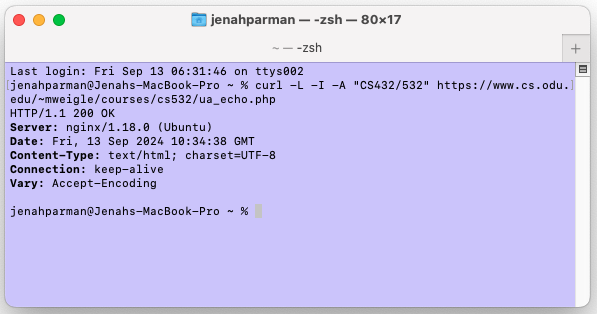
\includegraphics[width=0.5\linewidth]{q2_2.png}
    \caption{Screenshot of curl comand and result}
    \label{fig:q2_2}
\end{figure}


c) Use a single curl command with the appropriate options to do the following:

\begin{itemize}
    \item request the URI
    \item follow any redirects
    \item change the User-Agent HTTP request field to "CS432/532"
    \item save the HTML output to a file
\end{itemize}

Take a screenshot of the curl command and options you used and the result of your execution to include in your report.

\begin{figure}[!ht]
    \centering
    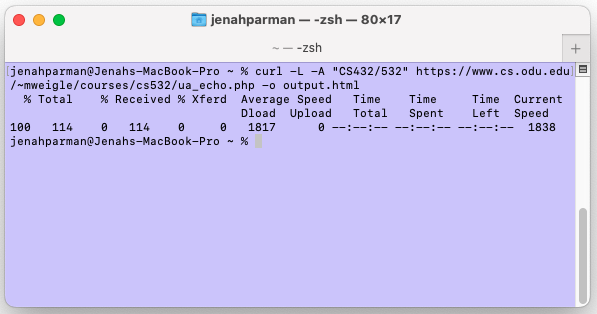
\includegraphics[width=0.5\linewidth]{q2_3.png}
    \caption{Screenshot of curl command and result of execution}
    \label{fig:q2_3}
\end{figure}

d) View the HTML output file that was produced by curl from part c in a web browser and take a screenshot to include in your report.

\begin{figure}[!ht]
    \centering
    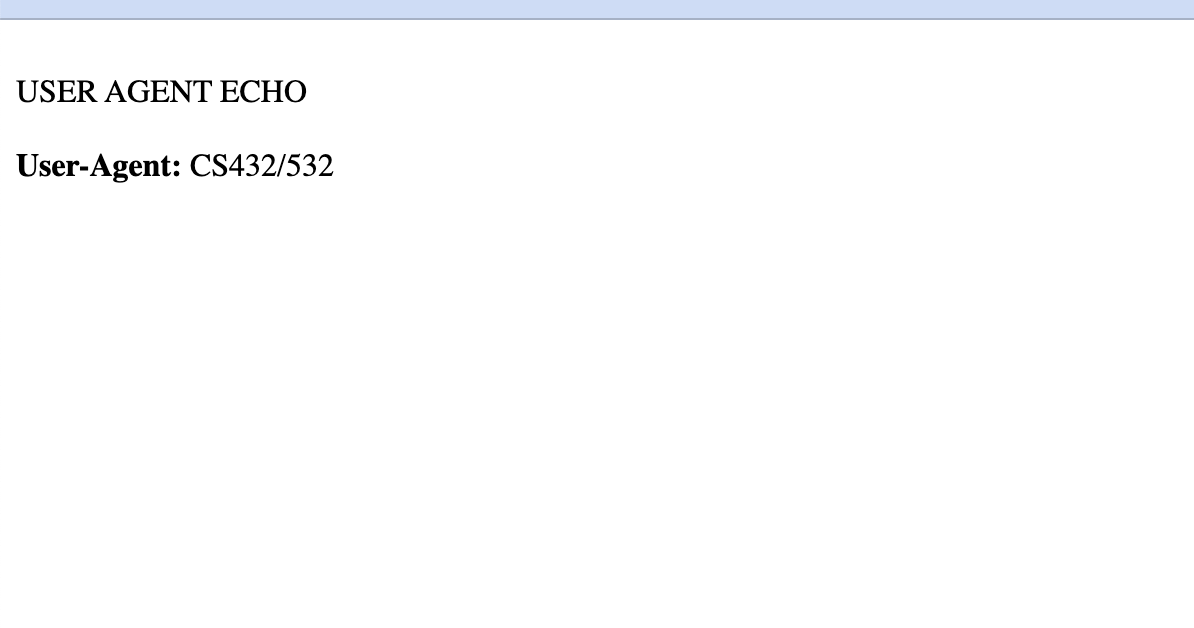
\includegraphics[width=0.5\linewidth]{q2_4.png}
    \caption{Screenshot of HTML output file that was produced by curl from part c in web browser}
    \label{fig:q2_4}
\end{figure}



\section*{Q3}

\begin{lstlisting}
import requests
from bs4 import BeautifulSoup

seed_uri = "https://en.wikipedia.org/wiki/2024_United_States_presidential_election"  # Starting URL
unique_uris = set()
to_crawl = [seed_uri]  # Start with the initial seed URL

def get_links(uri):
    try:
        response = requests.get(uri, timeout=5)
        if 'text/html' in response.headers.get('Content-Type', ''):
            soup = BeautifulSoup(response.text, 'html.parser')
            return [a['href'] for a in soup.find_all('a', href=True)]
    except requests.exceptions.RequestException:
        return []
    return []

def check_uri(uri):
    try:
        response = requests.get(uri, timeout=5)
        if 'text/html' in response.headers.get('Content-Type', ''):
            content_length = response.headers.get('Content-Length')
            if content_length and int(content_length) > 1000:
                return response.url
            elif len(response.content) > 1000:
                return response.url
    except requests.exceptions.RequestException:
        return None
    return None

# Keep collecting links until we hit 500 unique ones
while len(unique_uris) < 500 and to_crawl:
    current_seed = to_crawl.pop(0)  # Take the next URL to crawl
    seed_links = get_links(current_seed)
    for link in seed_links:
        if not link.startswith("http"):
            link = "https://en.wikipedia.org" + link  # Adjust for relative links
        final_uri = check_uri(link)
        if final_uri and final_uri not in unique_uris:
            unique_uris.add(final_uri)
            print(f"Collected: {len(unique_uris)} - {final_uri}")
            to_crawl.append(final_uri)  # Add new valid link to the crawl list
        if len(unique_uris) >= 500:
            break

# Save the collected URIs to a file
with open('collected_uris.txt', 'w') as file:
    for uri in unique_uris:
        file.write(uri + '\n')

print("Collected URIs saved to collected_uris.txt")

\end{lstlisting}

The Python program uses the second method (have your program randomly pick a URI that you've collected and use that as the new seed until you've collected 500 unique URIs) to collect 500 unique URIs from webpages. It starts with a seed URL, extracts all links from the page using BeautifulSoup, and checks if each link points to an HTML page with a content size greater than 1000 bytes. The program automatically selects new links from the collected URIs and continues crawling deeper into new pages until it reaches 500 unique URIs. This process is automated, requiring no manual intervention after the initial seed, making it an efficient way to gather the required data.

\section*{References}

\begin{itemize}
    \item {Overleaf, Code Listing \url{https://www.overleaf.com/learn/latex/Code_listing}}
    \item{Python Requests, \url{https://docs.python-requests.org/en/latest/user/quickstart/}}
    \item{Beautiful Soup Documentation, \url{https://www.crummy.com/software/BeautifulSoup/bs4/doc/}}
\end{itemize}

\end{document}

